% \section{Seed counter}
% \begin{figure}
%     \centering
%     \begin{subfigure}[t]{0.2\textwidth}
%         \centering
%         \includegraphics[width=0.6in]{counter_read_start_seed_case3_middle_level}
%         \caption{\label{fig:counter_read_start_seed_case3_middle_level} A ``clean'' counter row, before any reading has started.}
%     \end{subfigure}%
%     ~
%     \begin{subfigure}[t]{0.2\textwidth}
%         \centering
%         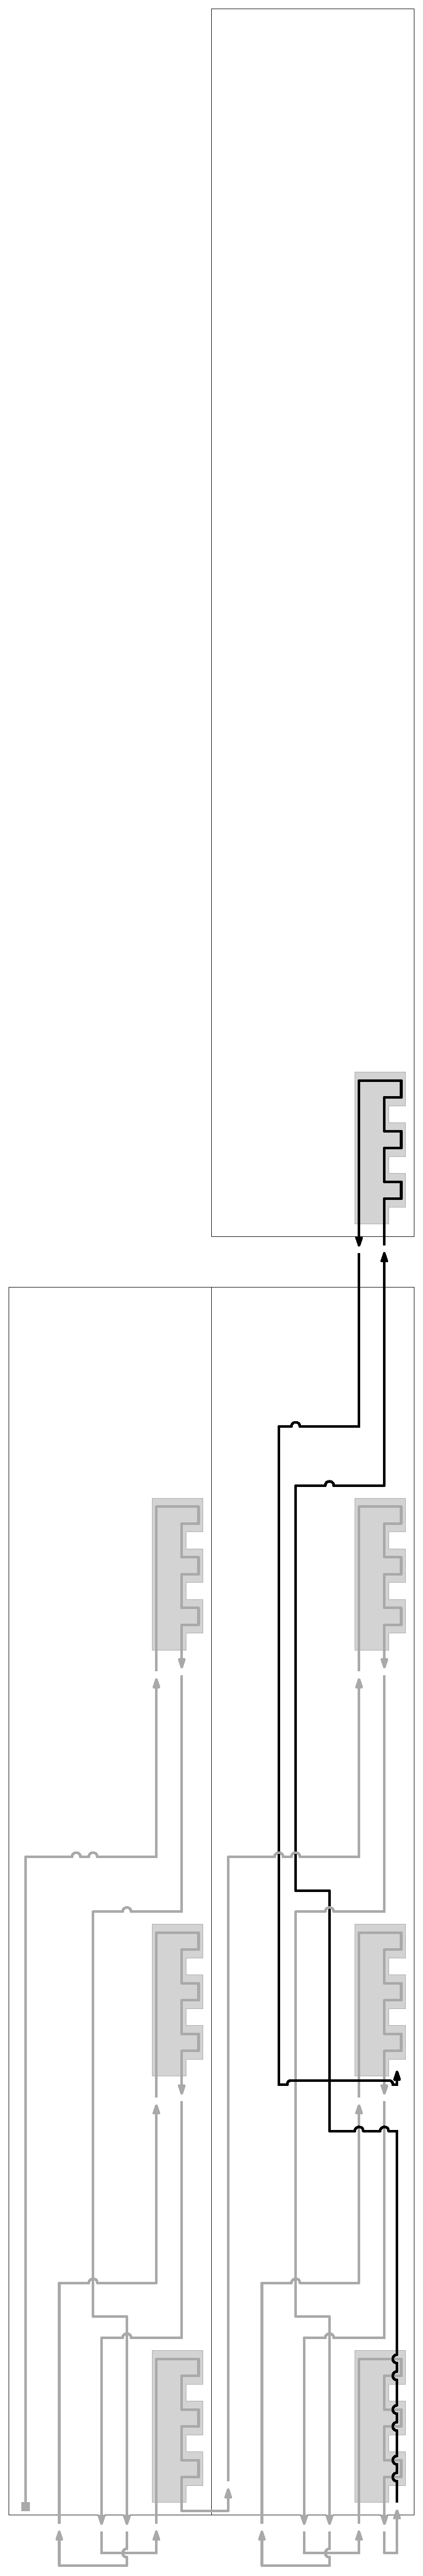
\includegraphics[width=0.6in]{counter_read_digit1_return_read_digit2_seed_case3_middle_level}
%         \caption{\label{fig:counter_read_digit1_return_read_digit2_seed_case3_middle_level} Reading digit 1, writing digit 1 in the next row, and returning to read digit 2 of the current row. }
%     \end{subfigure}%
%     ~
%     \begin{subfigure}[t]{0.2\textwidth}
%         \centering
%         \includegraphics[width=0.6in]{counter_read_digit2_return_read_digit3_seed_case3_middle_level}
%         \caption{\label{fig:counter_read_digit2_return_read_digit3_seed_case3_middle_level} Reading digit 2, writing digit 2 in the next row, and returning to read digit 3 of the current row. }
%     \end{subfigure}%
%     ~
%     \begin{subfigure}[t]{0.2\textwidth}
%         \centering
%         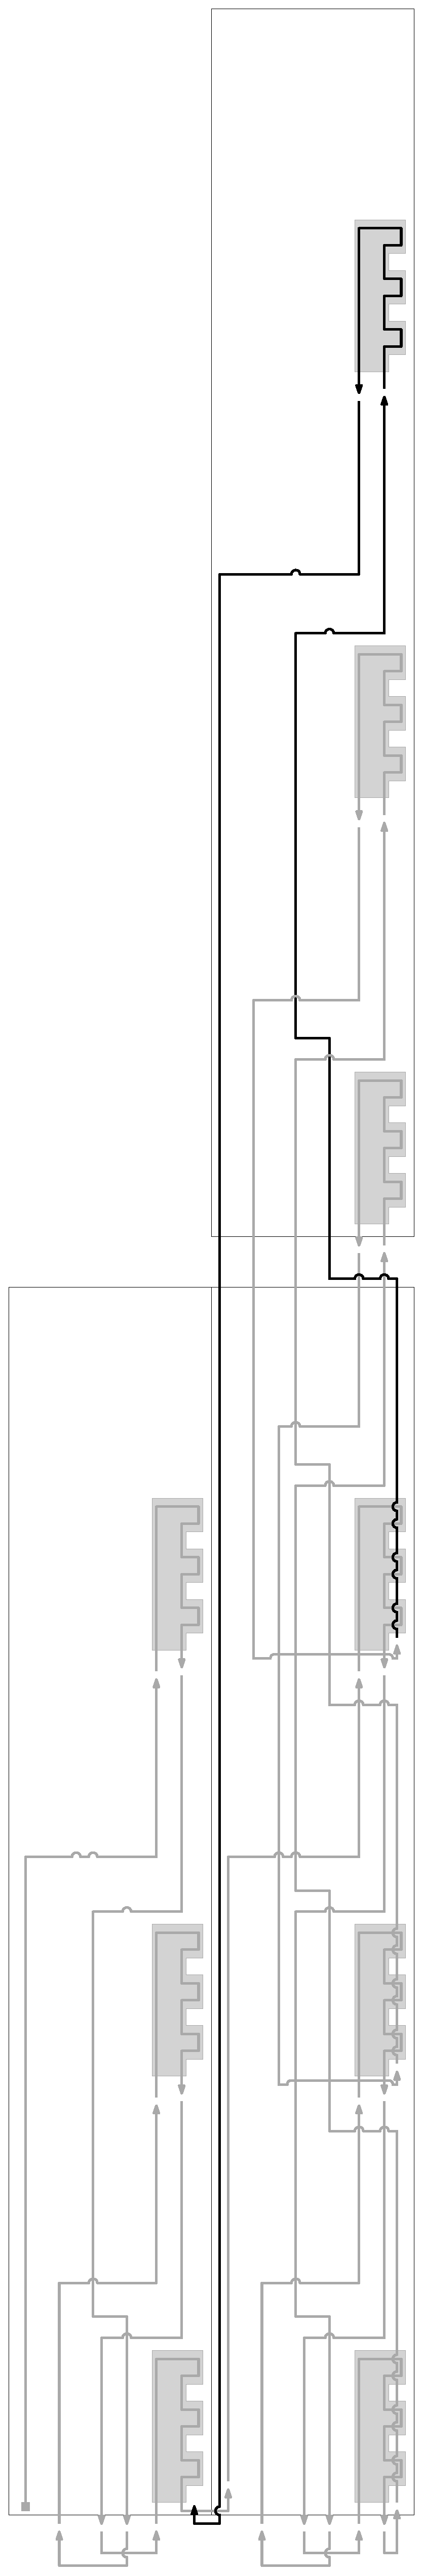
\includegraphics[width=0.6in]{counter_read_digit3_return_read_digit1_seed_case3_middle_level}
%         \caption{\label{fig:counter_read_digit3_return_read_digit1_seed_case3_middle_level} Reading digit 3, writing digit 3 in the next row, and returning to read digit 4 of the current row.}
%     \end{subfigure}%

%     \caption{\label{fig:counter_read_digit_return_read_digit_seed_case3} Progression of the counter as it reads the 3 least significant digits in one value, and writes the corresponding digits in the next row/value.}
% \end{figure}


\section{General counter}


\begin{figure}[H]
    \centering
    \begin{subfigure}[t]{0.2\textwidth}
        \centering
        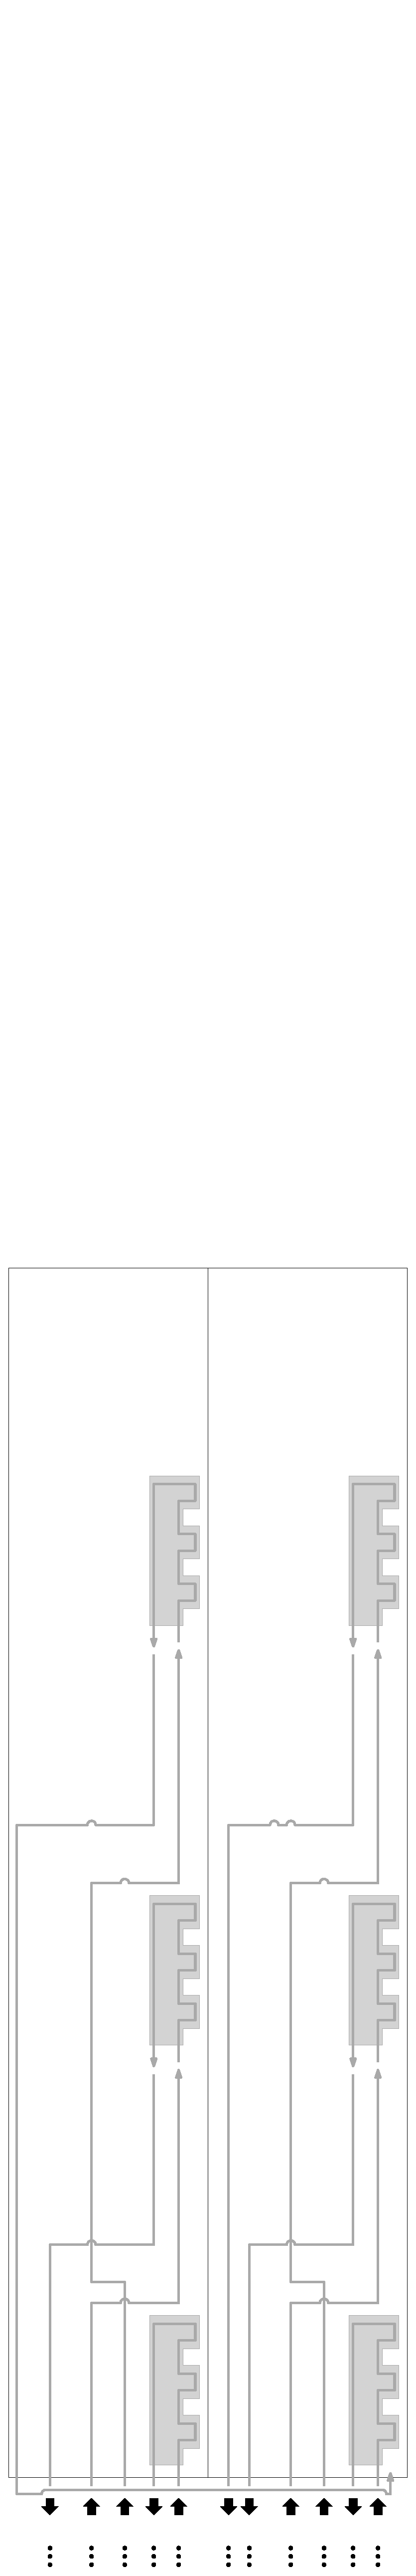
\includegraphics[width=0.6in]{counter_read_start_general_case3_middle_level}
        \caption{\label{fig:counter_read_start_general_case3_middle_level} A ``clean'' counter row, before any reading has started.}
    \end{subfigure}%
    ~
    \begin{subfigure}[t]{0.2\textwidth}
        \centering
        \includegraphics[width=0.6in]{counter_read_digit1_return_read_digit2_general_case3_middle_level}
        \caption{\label{fig:counter_read_digit1_return_read_digit2_general_case3_middle_level} Reading digit 1, writing digit 1 in the next row, and returning to read digit 2 of the current row. }
    \end{subfigure}%
    ~
    \begin{subfigure}[t]{0.2\textwidth}
        \centering
        \includegraphics[width=0.6in]{counter_read_digit2_return_read_digit3_general_case3_middle_level}
        \caption{\label{fig:counter_read_digit2_return_read_digit3_general_case3_middle_level} Reading digit 2, writing digit 2 in the next row, and returning to read digit 3 of the current row. }
    \end{subfigure}%
    ~
    \begin{subfigure}[t]{0.2\textwidth}
        \centering
        \includegraphics[width=0.6in]{counter_read_digit3_return_read_digit1_general_case3_middle_level}
        \caption{\label{fig:counter_read_digit3_return_read_digit1_general_case3_middle_level} Reading digit 3, writing digit 3 in the next row, and returning to read digit 4 of the current row.}
    \end{subfigure}%

    \caption{\label{fig:counter_read_digit_return_read_digit_general_case3} Progression of the counter as it reads the 3 least significant digits in one value, and writes the corresponding digits in the next row/value.}
\end{figure}
